\chapter{Quantum circuits}
\thispagestyle{chapterBeginStyle}
\label{chapter2}

In the previous chapter we introduced a new concept called \textbf{quantum circuit}. In this chapter, we will describe it in detail, which will enable us to create algorithms, which will be presented in the next chapter.

\section{Qubits}

In classical computers information is stored using \textbf{bits}. These entities can be in two states - 0 or 1. Thanks to this, we can encode any information as a string of bits in appropriate states.

In the example \ref{example_0_1_states} from the previous chapter we introduced two vectors (states) - $|0\rangle = \begin{pmatrix} 1 \\ 0 \end{pmatrix}$ and $|1\rangle = \begin{pmatrix} 0 \\ 1 \end{pmatrix}$. These two states can be quantum equivalents of classical states 0 and 1. They are orthonormal
\[ \langle 0 | 1 \rangle = \begin{pmatrix} 1 & 0\end{pmatrix} \begin{pmatrix} 0 \\ 1 \end{pmatrix} = 1 \cdot 0 + 0 \cdot 1 = 0,\]
so they can create a basis for a vector in Hilbert space. Hence, such a vector can be represented as a combination of these two states
\[ |\psi \rangle = \alpha |0\rangle + \beta |1\rangle. \]

The above vector is the basic information unit in quantum computer science - \textbf{qubit}. Comparing to classical bit, which can be only in 2 states, qubit can be in an infinite number of states (because it can be in any combination of states $|0\rangle$ and $|1\rangle$). Such a vector can be represented on the \textbf{Bloch sphere} (given below).

\begin{figure}[ht]
\centering
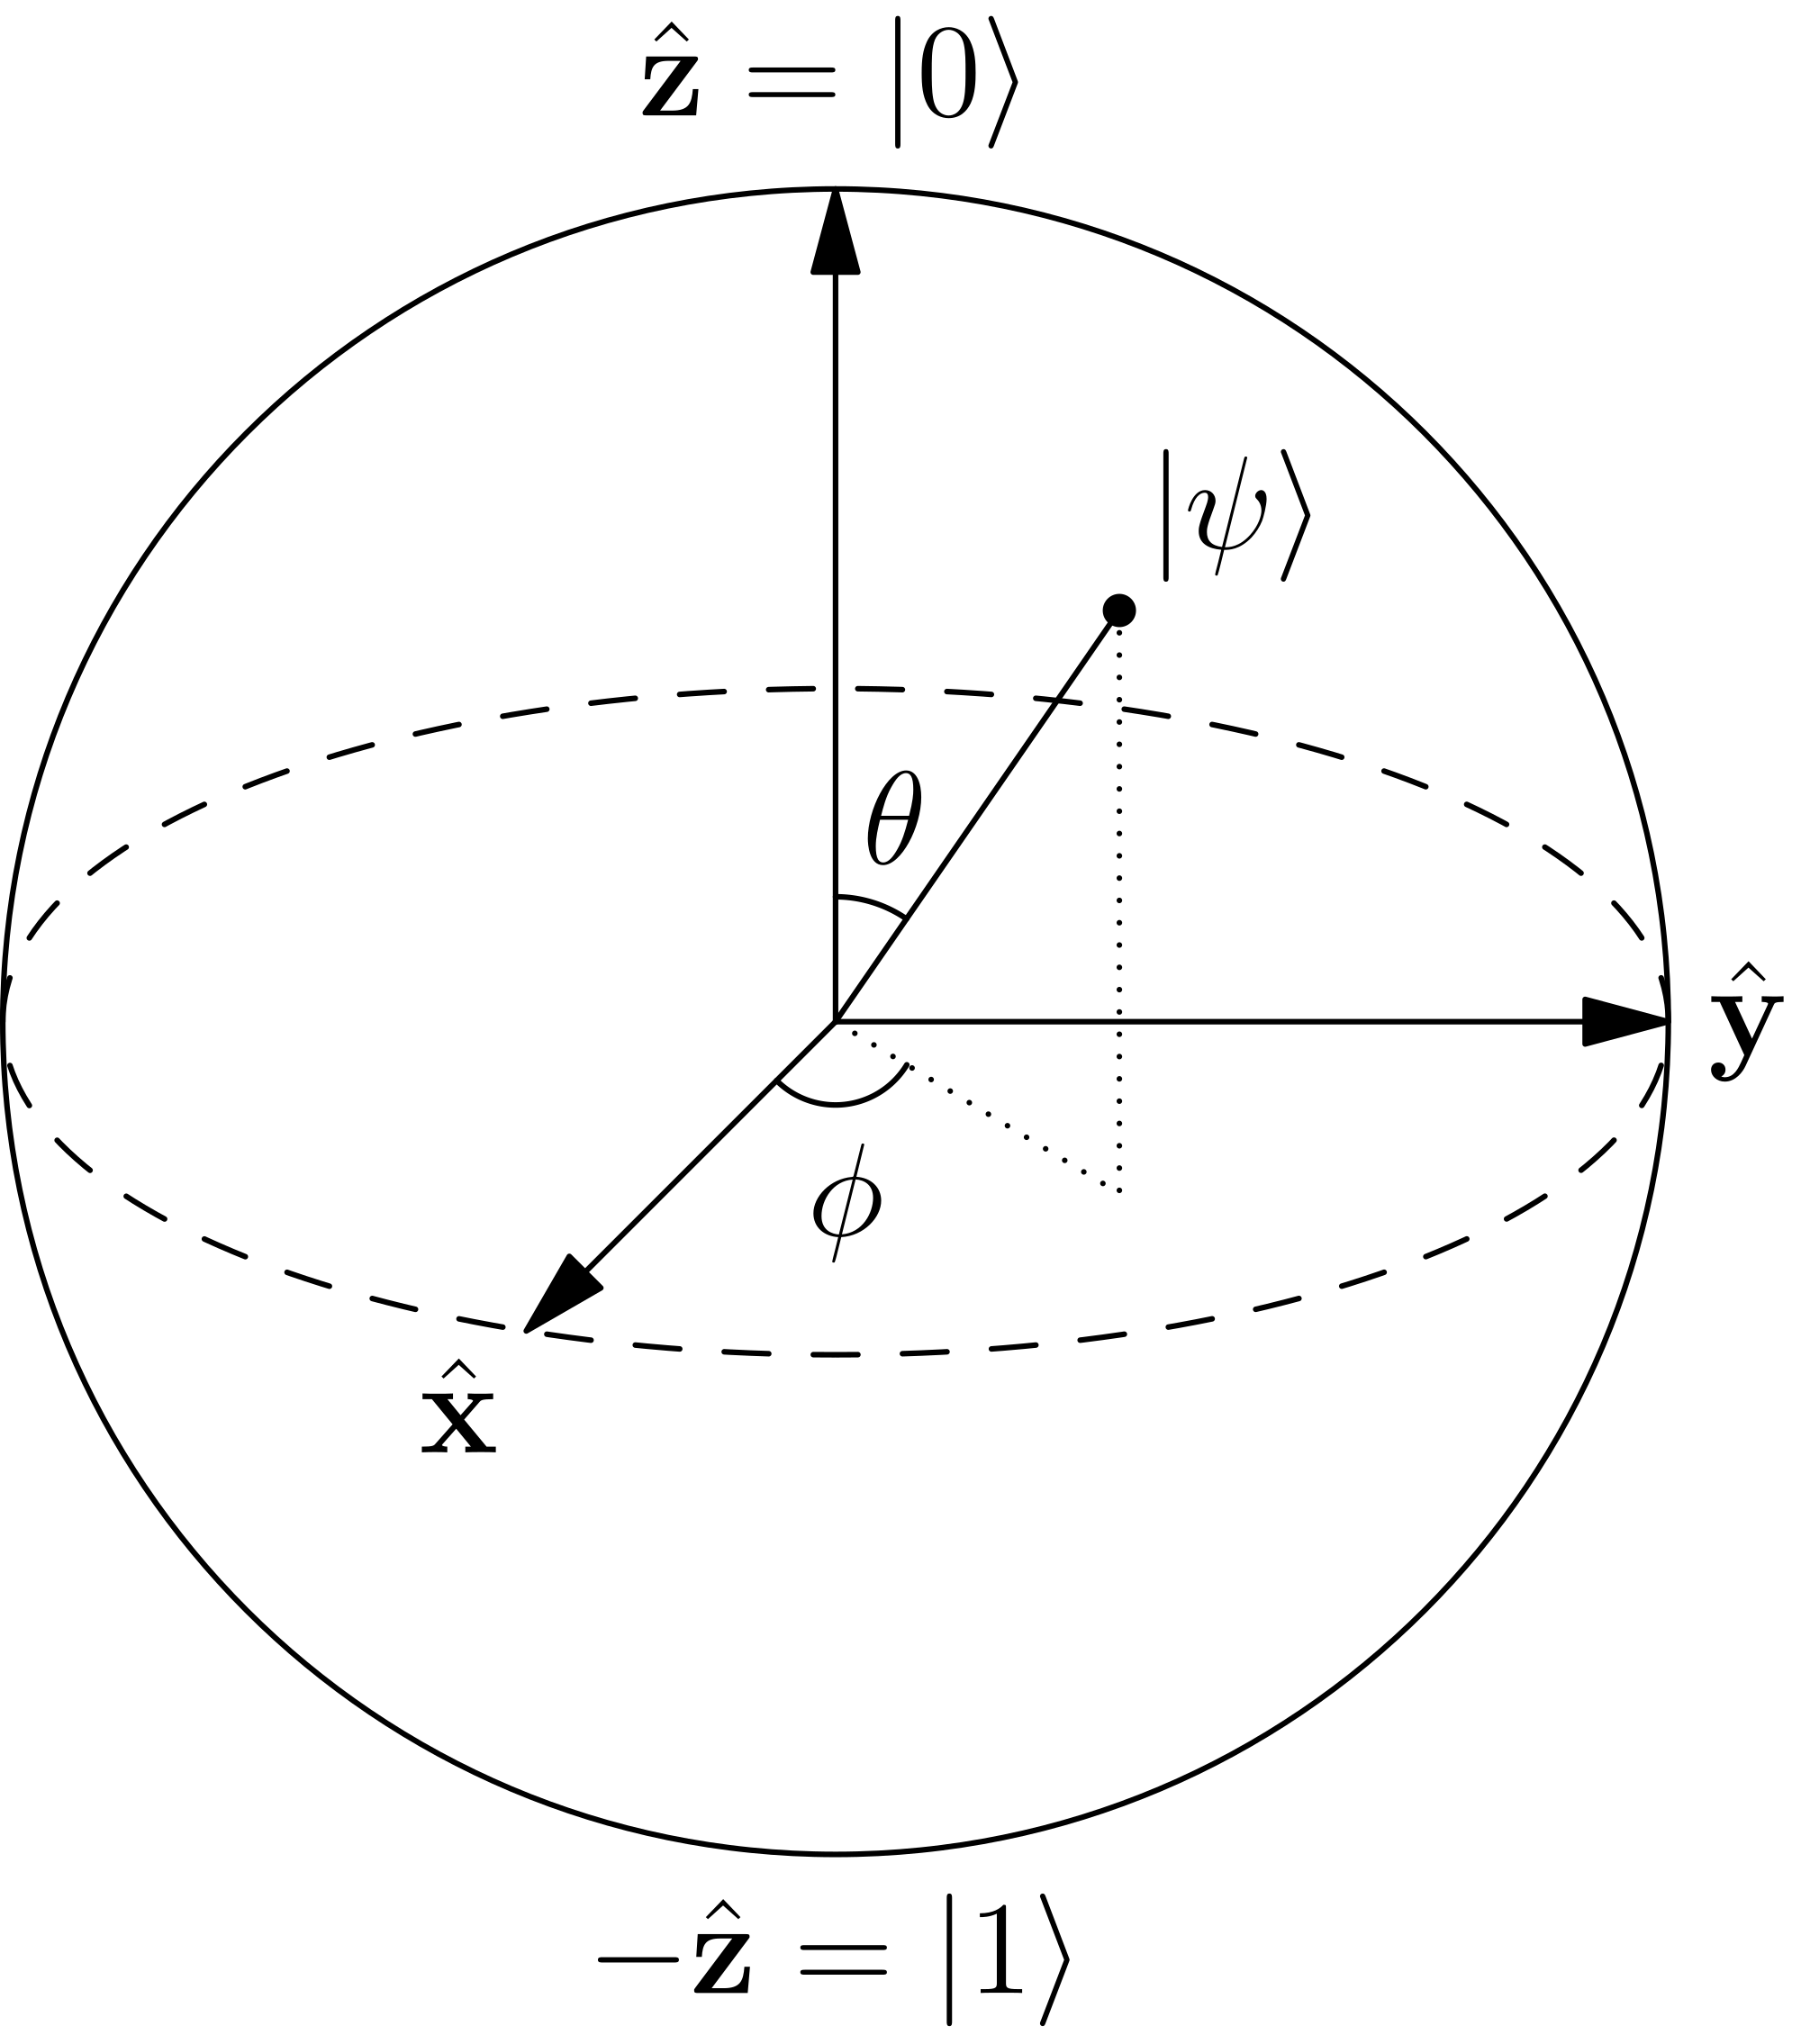
\includegraphics[scale=0.1]{bloch_sphere}
\caption{Representation of a qubit on the Bloch sphere.}
\end{figure}

The Bloch sphere gives a convenient way to show properties of a state vector. We have written, that a qubit can be expressed as a combination $|\psi\rangle = \alpha |0\rangle + \beta|1\rangle$. We also have a normalization constraint $|\alpha|^2 + |\beta|^2 = 1$. If squares of two probability amplitudes give 1, we can replace them with \textit{sin} and \textit{cos} functions of the same angle. Moreover, we cannot measure a global phase of a vector, but just a local one. Such local phase can be written as $e^{i \phi}$, where $\phi$ is some angle. When we combine all of the above we get

\[ |\psi\rangle = cos\bigg( \frac{\Theta}{2}\bigg)|0\rangle + sin\bigg( \frac{\Theta}{2}\bigg) e^{i \phi}|1\rangle.\]

Angles $\Theta$ and $\phi$ are shown in the picture above. Change in any of these angles can be easily seen on a sphere, which would not be as simple in a coordinate system, where states $|0\rangle$ and $|1\rangle$ are perpendicular.


\section{Reversible circuits}

A classical circuit can be considered as a \textbf{reversible} taking into account two criteria - \textit{physical} and \textit{logical} reversibility. In this work we will discuss only the second one.

A \textit{logically reversible circuit} is a circuit, in which action of each logical gate can be undone. In other words, we can restore the state of each bit, before the gate was applied.

A simple, classical, one bit logic gate - \textbf{NOT} gate is fully reversible. Let's say, we have a bit in the state 0 and apply the NOT gate to it. We receive a bit in the state 1. But during the whole procedure we didn't lose any information about the previous state of the considered bit. We can reverse this operation by applying another NOT gate and change bit's state from 1 to 0 (a NOT gate is it's own inverse gate).

Now, let's consider a two bit \textbf{OR} gate. It implements a simple logical operation

\begin{table}[ht]
    \centering
    \begin{tabular}{c|c|c}
         A & B & $A \vee B$ \\
         0 & 0 & 0 \\
         0 & 1 & 1 \\
         1 & 0 & 1 \\
         1 & 1 & 1
    \end{tabular}
    \caption{The action of the OR gate.}
    \label{tab:or_gate_action}
\end{table}

We can see, that if we apply this gate to two bits and receive 0, it is obvious, that these bits were in state 0. But if we receive 1 as an output it is impossible to determine, which one of them was in the state 1 (both of them could also be in this state). In the computing process we lost some information about the initial state of our two bits.

Quantum circuit is a version of a reversible circuit. In fact, each logic gate used in a quantum circuit can be considered as an unitary operator (or an unitary matrix). Thanks to this, an action of each quantum gate can be undone by applying the inverse gate.

\begin{remark}
A quantum gate can be its own inverse gate. If matrix \textit{U} is its own inverse ($U \equiv U^\dagger$) and $UU^\dagger = \mathbb{1}$, it is called \textit{unitary} and \textit{Hermitian}.  
\end{remark}

\section{Representation of a quantum circuit}

Quantum circuits will be presented in the further part of this work in the following way:

\begin{itemize}
    \item The time evolution of a circuit will be associated with the horizontal axis. Because of this, left side of each schema of a circuit will be the beginning of the computation,
    \item Each qubit will have assigned a horizontal line. It will demonstrate the time evolution of the qubits state,
    \item Quantum gates will be presented in the form of boxes.
\end{itemize}

An example quantum circuit is presented below:

\[  \scalebox{2.0}{\Qcircuit @C=1em @R=1em {
\lstick{|\psi\rangle} & \gate{H} & \targ & \meter  \\
\lstick{|\phi\rangle} & \qw & \ctrl{-1} & \meter \\
\lstick{|\theta\rangle} & {/^{n}} \qw & \gate{X} & \meter
}} \]

We will now discuss only two of the occurring in the above circuit symbols (rest of them will be explained in detail in next sections).

The symbol given below symbolizes a measurement of a qubit

\[ \scalebox{2.5}{\Qcircuit @C=1em @R=1em {
& \meter & \rstick{} \cw
}} \]

Sometimes we will replace many lines representing time evolution of many qubits' states using the following notation


\[ \scalebox{2.5}{\Qcircuit @C=1em @R=1em {
& {/^{n}} \qw & \qw
}} \]


\section{Single qubit quantum gates}

In contrast to the classical model of computation, we can create infinitely many single qubit quantum gates (in classic case we could only use the \textit{NOT} gate on one bit). It is possible, because we can associate each quantum gate with a rotation of the quantum state on the Bloch sphere. It is obvious, that we can make infinitely many different rotations, which proves our statement.

Below is given notation for chosen single qubit quantum gates, which will be used in this work.

\paragraph{Identity gate}

\[ I = \begin{pmatrix} 1 & 0 \\ 0 & 1 \end{pmatrix} \]

\paragraph{Pauli X gate (NOT gate)}

\[ X = \begin{pmatrix} 0 & 1 \\ 1 & 0 \end{pmatrix} \]

\paragraph{Pauli Z gate}

\[ Z = \begin{pmatrix} 1 & 0 \\ 0 & -1 \end{pmatrix} \]

\paragraph{Hadamard gate}

\[ H =  \frac{1}{\sqrt{2}} \begin{pmatrix} 1 & 1 \\ 1 & -1 \end{pmatrix} \]

\paragraph{Phase shift ($R_k$ gate)}

\[ R_k = \begin{pmatrix} 1 & 0 \\ 0 & e^{\frac{2 \pi i}{2^k}} \end{pmatrix} \]

\begin{remark}
In literature the gate $R_k$ is often replaced with the $R_\phi$ gate, which is equivalent to

\[ R_\phi = \begin{pmatrix} 1 & 0 \\ 0 & e^{i \phi} \end{pmatrix}. \]

Despite this fact, we will use only the $R_k$ gate.
\end{remark}

\begin{remark}
As stated in the first chapter, when we are considering a complex physical system (made for example from two qubits) we are using the tensor product of the two component subsystems. Let's see this at the quantum circuit given below.

\[  \scalebox{2.0}{\Qcircuit @C=1em @R=1em {
\lstick{|\psi\rangle} & \gate{H} & \rstick{|\psi'\rangle} \qw \\
\lstick{|\phi\rangle} & \gate{I} & \rstick{|\phi'\rangle} \qw \\
}} \]

If we would like to replace the gates \textit{H} and \textit{I} with just one gate (let's call it \textit{C}) we would have to conduct the following procedure

\[ C = H \otimes I = \frac{1}{\sqrt{2}} \begin{pmatrix} 1 & 1 \\ 1 & -1 \end{pmatrix} \otimes \begin{pmatrix} 1 & 0 \\ 0 & 1\end{pmatrix} = \frac{1}{\sqrt{2}} \begin{pmatrix} 1 & 0 & 1 & 0 \\ 0 & 1 & 0 & 1 \\ 1 & 0 & -1 & 0 \\ 0 & 1 & 0 & -1 \end{pmatrix}.\]

We can see, that we can replace the \textit{C} gate with just \textbf{one layer} of smaller quantum gates. But it is not always possible. We will give an example of such a case in the next section.
\end{remark}

\section{Multiple qubit quantum gates}

In the first chapter we stated, that not all compound systems can be expressed in the form of tensor product of its subsystems. We called this phenomenon \textit{entanglement}. This property of quantum entities is often used in quantum computing. Using entanglement we can create \textbf{controlled gates}. A simple example of a controlled gate is the \textbf{controlled-NOT} gate (sometimes denoted as \textbf{CNOT}). In the matrix form it is written as

\[ CNOT = \begin{pmatrix} 1 & 0 & 0 & 0 \\ 0 & 1 & 0 & 0 \\ 0 & 0 & 0 & 1 \\ 0 & 0 & 1 & 0 \end{pmatrix} \]

We can see, that we cannot receive such a matrix as a result of tensor product of smaller matrices.

The \textit{CNOT} gate is represented in quantum circuits by the symbol

\[  \scalebox{2.0}{\Qcircuit @C=1em @R=1em {
 & \ctrl{1} & \qw \\
 & \targ & \qw \\
}} \]

The upper qubit is called a \textbf{control} qubit, and the bottom qubit is referred as to \textbf{target} qubit. To better understand what this quantum gate does, let's consider the following circuit

\[  \scalebox{2.0}{\Qcircuit @C=1em @R=1em {
\lstick{|\psi\rangle} & \ctrl{1} & \rstick{|\psi\rangle} \qw \\
\lstick{|\phi\rangle} & \targ & \rstick{|\phi \oplus \psi \rangle} \qw \\
}} \]

The \textit{CNOT} gate performs some operation (we will describe this operation in a moment), when the control qubit is in state $|1\rangle$. Otherwise, the whole system is left without any change.

In fact, the \textit{CNOT} gate can be understood as follows - it leaves the control qubit in the same state, and the bottom qubit becomes the result of \textit{addition modulo two} of the two qubits' states. Let's say, we have qubits in states $|0\rangle$ and $|1\rangle$ (accordingly control and target qubits). The usage of \textit{CNOT} gate can be written as

\[ CNOT |0\rangle \otimes |1\rangle = CNOT \begin{pmatrix} 1 \\ 0 \end{pmatrix} \otimes \begin{pmatrix} 0 \\ 1 \end{pmatrix} = \begin{pmatrix} 1 & 0 & 0 & 0 \\ 0 & 1 & 0 & 0 \\ 0 & 0 & 0 & 1 \\ 0 & 0 & 1 & 0 \end{pmatrix} \begin{pmatrix} 0 \\ 1 \\ 0 \\ 0 \end{pmatrix} = \begin{pmatrix} 0 \\ 1 \\ 0 \\ 0\end{pmatrix} = |0\rangle \otimes |1\rangle.\]

Now, let's consider qubits in states $|1\rangle$ and $|1\rangle$. The result of the above circuit for qubits in such states is equal to

\[ CNOT |1\rangle \otimes |1\rangle = CNOT \begin{pmatrix} 0 \\ 1 \end{pmatrix} \otimes \begin{pmatrix} 0 \\ 1 \end{pmatrix} = \begin{pmatrix} 1 & 0 & 0 & 0 \\ 0 & 1 & 0 & 0 \\ 0 & 0 & 0 & 1 \\ 0 & 0 & 1 & 0 \end{pmatrix} \begin{pmatrix} 0 \\ 0 \\ 0 \\ 1 \end{pmatrix} = \begin{pmatrix} 0 \\ 0 \\ 1 \\ 0 \end{pmatrix} = |1\rangle \otimes |0\rangle.\]

It is obvious, that $0 + 1 \ (mod \ 2) \equiv 1$ and $1 + 1 \ (mod \ 2) \equiv 0$, so we have shown, that understanding of the \textit{CNOT} gate in terms of the modular addition is correct. All possible results of the \textit{CNOT} gate are given in the table below.

\begin{table}[ht]
    \centering
    \begin{tabular}{c|c|c}
         $|\psi\rangle$ & $|\phi\rangle$ & $CNOT \  |\psi \phi \rangle$ \\ \hline
         $|0\rangle$ & $|0\rangle$ & $|00\rangle$ \\
         $|0\rangle$ & $|1\rangle$ & $|01\rangle$ \\
         $|1\rangle$ & $|0\rangle$ & $|11\rangle$ \\
         $|1\rangle$ & $|1\rangle$ & $|10\rangle$ \\
    \end{tabular}
    \caption{Actions of the \textit{CNOT} gate.}
    \label{tab:my_label}
\end{table}

The \textit{CNOT} gate is a simple extension of the \textit{NOT} gate. We can see, that the bottom right block of the \textit{CNOT} matrix is just the \textit{X} matrix. We can extend this reasoning, to create a whole class of controlled gates. Let's say, we have some quantum gate \textit{M} in the form

\[ M = \begin{pmatrix} m_{11} & m_{12} \\ m_{21} & m_{22}\end{pmatrix}. \]

The controlled version of this gate would have a form

\[ cM = \begin{pmatrix} 1 & 0 & 0 & 0 \\ 0 & 1 & 0 & 0 \\ 0 & 0 & m_{11} & m_{12} \\ 0 & 0 & m_{21} & m_{22} \end{pmatrix}. \]

Of course we can extend the simple case with a $2 \times 2$ matrix to a matrix with many inputs (acting on many qubits). Such a case will be represented by symbol

\[  \scalebox{1.5}{\Qcircuit @C=1em @R=.5em {
& \ctrl{1} & \qw \\
& \multigate{3}{M} & \qw \\
& \ghost{M} & \qw \\
& \ghost{M} & \qw \\
& \ghost{M} & \qw
}} \]

or 

\[  \scalebox{2.0}{\Qcircuit @C=1em @R=.5em {
& \qw & \ctrl{1} & \qw \\
& {/^{n}} \qw & \gate{M} & \qw 
}} \]

\begin{remark}
As we can see from the below calculations

\[ \begin{pmatrix} 1 & 0 & 0 & 0 \\ 0 & 1 & 0 & 0 \\ 0 & 0 & 0 & 1 \\ 0 & 0 & 1 & 0 \end{pmatrix} \begin{pmatrix} 1 & 0 & 0 & 0 \\ 0 & 1 & 0 & 0 \\ 0 & 0 & 0 & 1 \\ 0 & 0 & 1 & 0 \end{pmatrix} = \begin{pmatrix} 1 & 0 & 0 & 0 \\ 0 & 1 & 0 & 0 \\ 0 & 0 & 1 & 0 \\ 0 & 0 & 0 & 1 \end{pmatrix} \]

the \textit{CNOT} gate is its own inverse gate.
\end{remark}

Out of three \textit{CNOT} gates we can create a \textit{SWAP} gate, which changes states between two qubits. It will be denoted as 

\[  \scalebox{2.5}{\Qcircuit @C=1em @R=1em {
& \qswap & \qw \\
& \qswap \qwx & \qw
}} \]

\[ \]

and can be implemented with the following circuit

\[  \scalebox{2.0}{\Qcircuit @C=1em @R=.5em {
& \lstick{|\psi\rangle} & \ctrl{1} & \targ & \ctrl{1} & \qw & \rstick{|\phi\rangle}\\
& \lstick{|\phi\rangle} & \targ & \ctrl{-1} & \targ & \qw & \rstick{|\psi\rangle}
}} \]

Consecutive steps of the above construction can be written as

\[ |\psi, \phi \rangle \rightarrow |\psi, \phi \oplus \psi\rangle \] 
\[ \rightarrow |\psi \oplus (\phi \oplus \psi), \phi \oplus \psi\rangle \equiv |\phi, \phi \oplus \psi \rangle \]
\[ \rightarrow |\phi, (\phi \oplus \psi) \oplus \phi \rangle \equiv |\phi, \psi \rangle, \]
where coma was added to increase the readability of the whole procedure.

\section{Bell states} \label{bell_states}

Let's consider the following circuit:

\[  \scalebox{2.0}{\Qcircuit @C=1em @R=.5em {
& \lstick{|x\rangle} & \gate{H} & \ctrl{1} & \qw \\
& \lstick{|y\rangle} & \qw & \targ & \qw 
}} \]

Assuming, that $|x\rangle$ was only in one of $|0\rangle$ and $|1\rangle$ states, usage of the first Hadamrd gate has two possible outcomes:

\[ |0\rangle \xrightarrow{H} \frac{|0\rangle + |1\rangle}{\sqrt{2}}\]
\[ |1\rangle \xrightarrow{H} \frac{|0\rangle - |1\rangle}{\sqrt{2}}\]

As mentioned before, the \textit{CNOT} gate is applied to the $|y\rangle$ qubit only, if the control qubit is in a state $|1\rangle$. So, if we have a control qubit being in a superposition, the target qubit will also be in a superposition of being toggled and unchanged. Let's denote by $|\beta_{xy}\rangle$ state of the whole system after going through the whole circuit. We present possible values of $|\beta_{xy}\rangle$ in the table below.

\begin{table}[ht]
    \centering
    \begin{tabular}{|c|c|c|}
        \hline
         \multicolumn{2}{|c|}{Input} & Output \\ \hline
         $|x\rangle$ & $|y\rangle$ & $|\beta_{xy}\rangle$ \\ \hline
         $|0\rangle$ & $|0\rangle$ & $(|00\rangle + |11\rangle)/\sqrt{2}$ \\ \hline
         $|0\rangle$ & $|1\rangle$ & $(|01\rangle + |10\rangle)/\sqrt{2}$ \\ \hline
         $|1\rangle$ & $|0\rangle$ & $(|00\rangle - |11\rangle)/\sqrt{2}$ \\ \hline
         $|1\rangle$ & $|1\rangle$ & $(|01\rangle - |10\rangle)/\sqrt{2}$ \\ \hline
    \end{tabular}
    \caption{Bell states.}
\end{table}

Received $|\beta_{xy}\rangle$ states are called \textbf{Bell states}.


\section{Quantum gates with multiple control qubits, ancilla qubits}

We can extend the controlled gate model by adding more control qubits. The simplest example of quantum gate with many control qubits is the \textbf{Toffoli} gate. It will be denoted as

\[  \scalebox{2.0}{\Qcircuit @C=1em @R=1em {
& \lstick{|\psi\rangle} & \ctrl{2} & \qw & \rstick{|\psi\rangle}  \\
& \lstick{|\phi\rangle} & \ctrl{1} & \qw & \rstick{|\phi\rangle}  \\
& \lstick{|\theta\rangle} & \targ & \qw & \rstick{|\theta \oplus \psi\phi\rangle} 
}} \]
\[\]
It's action is similar to the one of the \textit{CNOT} gate. It applies addition modulo two on the target qubit, if two control qubits are in the state $|1\rangle$. It's effect is presented in the table below.

\begin{table}[ht]
    \centering
    \begin{tabular}{c|c}
         Input & Output \\ \hline
         $|000\rangle$ & $|000\rangle$ \\
         $|001\rangle$ & $|001\rangle$ \\
         $|010\rangle$ & $|010\rangle$ \\
         $|011\rangle$ & $|011\rangle$ \\
         $|100\rangle$ & $|100\rangle$ \\
         $|101\rangle$ & $|101\rangle$ \\
         $|110\rangle$ & $|111\rangle$ \\
         $|111\rangle$ & $|110\rangle$ \\
    \end{tabular}
    \caption{Actions of the Toffoli gate.}
    \label{tab:my_label}
\end{table}

It can be written in the matrix form as

\[ \begin{pmatrix} 1 & 0 & 0 & 0 & 0 & 0 & 0 & 0 \\ 0 & 1 & 0 & 0 & 0 & 0 & 0 & 0 \\ 0 & 0 & 1 & 0 & 0 & 0 & 0 & 0 \\ 0 & 0 & 0 & 1 & 0 & 0 & 0 & 0 \\ 0 & 0 & 0 & 0 & 1 & 0 & 0 & 0 \\ 0 & 0 & 0 & 0 & 0 & 1 & 0 & 0 \\ 0 & 0 & 0 & 0 & 0 & 0 & 0 & 1 \\ 0 & 0 & 0 & 0 & 0 & 0 & 1 & 0 \end{pmatrix}. \]


\begin{remark}
At this point we will assume, that it is physically possible to implement \textit{CNOT} and Toffoli gates. Because of this assumption, we can try to break down more complicated gates into \textit{CNOT} and Toffoli gates. Toffoli gates are in fact universal gates, which will be explained in the next section.
\end{remark}

Of course we can add next control qubits and receive for example such gate:

\[  \scalebox{2.0}{\Qcircuit @C=1em @R=1em {
 & \ctrl{4} & \qw \\
 & \ctrl{3} & \qw \\
 & \ctrl{2} & \qw \\
 & \ctrl{1} & \qw \\
 & \gate{M} & \qw \\
}} \]

\begin{remark}
\textit{NOT} gates with more than two control qubits will be denoted as $C^n NOT$ gates (where \textit{n} is the number of control qubits).
\end{remark}

Unfortunately, it might be physically impossible to construct such a gate. But, as we mentioned in the above remark, we can break it down into \textit{CNOT} and Toffoli gates. To achieve this goal we will have to use \textbf{ancilla qubits}.

\subsection{Ancilla qubits}

Ancilla qubits are additional qubits, which expand our work space. They can be, for example, taken from some other part of a quantum circuit, where they are currently not used. Because of this, it is sometimes necessary to return them in unchanged state to the original location in the circuit.

We will now introduce four types of ancilla qubits. Although this notation is not officially used (it was taken from \cite{craig_gidney}), we will use it, because it perfectly captures the nature of each ancilla qubit type.

\begin{itemize}
    \item \textbf{Burnable qubits} - initially, those qubits are in state $|0\rangle$ and there are no requirements about the state, in which it is to be found at the end of the computation.
    \item \textbf{Zeroed qubits} - initially they are in state $|0\rangle$ and have to be in this state, when we are not going to use them any more.
    \item \textbf{Garbage qubits} - the initial state of these qubits is unknown and there are no restrictions concerning the final state.
    \item \textbf{Borrowed qubits} - at the beginning of the computation they can be in any state and have to be returned in the same state.
\end{itemize}

\begin{remark}
We will use the following notation to denote different types of ancilla qubits:
\begin{itemize}
    \item $|BU_i\rangle$ for burnable qubits,
    \item $|Z_i\rangle$ for zeroed qubits,
    \item $|G_i\rangle$ for garbage qubits,
    \item $|BO_i\rangle$ for borrowed qubits,
\end{itemize}
where \textit{i} will be the index for the following ancilla qubits.
\end{remark}

\subsection{Decomposition of the $C^n NOT$ gate into $C^{n/2}NOT$ gates}

Our first goal is to break down the below gate into more gates with fewer control qubits.

\[  \scalebox{1.5}{\Qcircuit @C=1em @R=1em {
& \lstick{|a\rangle} & \ctrl{4} & \qw & \rstick{|a\rangle}  \\
& \lstick{|b\rangle} & \ctrl{3} & \qw & \rstick{|b\rangle}  \\
& \lstick{|c\rangle} & \ctrl{2} & \qw & \rstick{|c\rangle}  \\
& \lstick{|d\rangle} & \ctrl{1} & \qw & \rstick{|d\rangle}  \\
& \lstick{|T\rangle} & \targ & \qw & \rstick{|T \oplus abcd\rangle} 
}} \]

\paragraph{Decomposition of the $C^n NOT$ gate with one burnable qubit \\}

If we have one additional burnable qubit to use, we can toggle it, if half of the control qubits are in state $|1\rangle$. As a result we obtain the following circuit:

\[  \scalebox{1.5}{\Qcircuit @C=1em @R=1em {
& \lstick{|a\rangle} & \ctrl{4} & \qw & \qw & \rstick{|a\rangle}  \\
& \lstick{|b\rangle} & \ctrl{3} & \qw & \qw & \rstick{|b\rangle}  \\
& \lstick{|c\rangle} & \qw & \ctrl{3} & \qw & \rstick{|c\rangle}  \\
& \lstick{|d\rangle} & \qw & \ctrl{2} & \qw & \rstick{|d\rangle}  \\
& \lstick{|BU_1\rangle} & \targ & \ctrl{1} & \qw & \rstick{|0 \oplus ab\rangle = |ab\rangle}  \\
& \lstick{|T\rangle} & \qw & \targ & \qw & \rstick{|T \oplus abcd\rangle} 
}} \]

\paragraph{Decomposition of the $C^n NOT$ gate with one zeroed qubit \\}

At the end of the previous section we have shown, that the \textit{CNOT} gate is its own inverse gate. In fact, any $C^nNOT$ gate is its own inverse gate. We will use this property, while using the \textit{zeroed} qubit. If we apply the $C^nNOT$ gate to this ancilla qubit for the first time, its state might change. But we can cancel the action of the first gate by using the $C^nNOT$ gate second time. This reasoning gives us the following quantum circuit:

\[  \scalebox{1.5}{\Qcircuit @C=1em @R=1em {
& \lstick{|a\rangle} & \ctrl{4} & \qw & \ctrl{4} & \qw & \rstick{|a\rangle}  \\
& \lstick{|b\rangle} & \ctrl{3} & \qw & \ctrl{3} & \qw & \rstick{|b\rangle}  \\
& \lstick{|c\rangle} & \qw & \ctrl{3} & \qw & \qw & \rstick{|c\rangle}  \\
& \lstick{|d\rangle} & \qw & \ctrl{2} & \qw & \qw & \rstick{|d\rangle}  \\
& \lstick{|Z_1\rangle} & \targ & \ctrl{1} &\targ & \qw & \rstick{|Z_1\rangle = |0\rangle}  \\
& \lstick{|T\rangle} & \qw & \targ & \qw & \qw & \rstick{|T \oplus abcd\rangle} 
}} \]

\paragraph{Decomposition of the $C^n NOT$ gate with one garbage qubit \\}

Because we do not know the initial state of the garbage qubit, the only way for us do detect any behavior is to check, whether it was toggled or not. The \textit{modular addition} (or \textit{XOR} operation) has such property, that if we use it two times with the same argument, these operations cancel out. This can be written as

\[ x \oplus y \oplus y \equiv x.  \]

This property gives us the following structure

\[  \scalebox{1.5}{\Qcircuit @C=1em @R=1em {
& \lstick{|a\rangle} & \qw & \ctrl{4} & \qw & \qw & \rstick{|a\rangle}  \\
& \lstick{|b\rangle} & \qw & \ctrl{3} & \qw & \qw & \rstick{|b\rangle}  \\
& \lstick{|c\rangle} & \ctrl{3} & \qw & \ctrl{3} & \qw & \rstick{|c\rangle}  \\
& \lstick{|d\rangle} & \ctrl{2} & \qw & \ctrl{2} & \qw & \rstick{|d\rangle}  \\
& \lstick{|G_1\rangle} & \ctrl{1} &\targ & \ctrl{1} & \qw & \rstick{|G_1 \oplus ab \rangle}  \\
& \lstick{|T\rangle} & \targ & \qw & \targ & \qw & \rstick{|T \oplus abcd\rangle} 
}} \]

We can see, that we are adding $|G_1\rangle$ to $|T\rangle$ two times, so these operations cancel out. The only possible leftover of this procedure is $|T \oplus ab\rangle$. Finally, the result of the whole above circuit can be written as

\[ |T \oplus G_1cd \oplus (G_1 \oplus ab)cd \rangle \equiv |T \oplus (G_1 \oplus G_1 \oplus ab)cd \rangle \equiv |T \oplus abcd \rangle\]

\paragraph{Decomposition of the $C^n NOT$ gate with one borrowed qubit \\}

The last case is very similar to the previous one (with garbage qubit). We only have to detect the possible toggling of the borrowed qubit and moreover, we have to undo the operation applied on it, to restore it to its initial state. It can be done using the below circuit

\[  \scalebox{1.5}{\Qcircuit @C=1em @R=1em {
& \lstick{|a\rangle} & \ctrl{4} & \qw & \ctrl{4} & \qw & \qw & \rstick{|a\rangle}  \\
& \lstick{|b\rangle} & \ctrl{3} & \qw & \ctrl{3} & \qw & \qw & \rstick{|b\rangle}  \\
& \lstick{|c\rangle} & \qw & \ctrl{3} & \qw & \ctrl{3} & \qw & \rstick{|c\rangle}  \\
& \lstick{|d\rangle} & \qw & \ctrl{2} & \qw & \ctrl{2} & \qw & \rstick{|d\rangle}  \\
& \lstick{|BO_1\rangle} & \targ & \ctrl{1} &\targ & \ctrl{1} & \qw & \rstick{|BO_1\rangle}  \\
& \lstick{|T\rangle} & \qw & \targ & \qw & \targ & \qw & \rstick{|T \oplus abcd\rangle} 
}} \]

\subsection{Decomposition of the $C^nNOT$ gate using \textit{n - 2} ancilla qubits}

We stated in the previous section, that it is possible to physically implement Toffoli gates. We will now try to break down $C^nNOT$ gate using different types of ancilla qubits and Toffoli gates.

In presented circuits we will interleave basic and ancilla qubits in order to increase the readability of diagrams. We will use constructions derived in the previous subsection and only show diagrams representing decomposed $C^nNOTs$.

\paragraph{Decomposition of the $C^nNOT$ gate using burnable qubits\\}

\[ \scalebox{1.3}{\Qcircuit @C=1em @R=1em {
& \lstick{|a\rangle} & \ctrl{2} & \qw & \qw & \qw & \qw & \rstick{|a\rangle} \\
& \lstick{|b\rangle} & \ctrl{1} & \qw & \qw & \qw & \qw & \rstick{|b\rangle} \\
& \lstick{|BU_1\rangle} & \targ & \ctrl{2} & \qw & \qw & \qw & \rstick{|ab\rangle} \\
& \lstick{|c\rangle} & \qw & \ctrl{1} & \qw & \qw & \qw & \rstick{|c\rangle} \\
& \lstick{|BU_2\rangle} & \qw & \targ & \ctrl{2} & \qw & \qw & \rstick{|abc\rangle} \\
& \lstick{|d\rangle} & \qw & \qw & \ctrl{1} & \qw & \qw & \rstick{|d\rangle} \\
& \lstick{|BU_3\rangle} & \qw & \qw & \targ & \ctrl{2} & \qw & \rstick{|abcd\rangle} \\
& \lstick{|e\rangle} & \qw & \qw & \qw & \ctrl{1} & \qw & \rstick{|e\rangle} \\
& \lstick{|T\rangle} & \qw & \qw & \qw & \targ & \qw & \rstick{|T \oplus abcde\rangle} 
}} \]

\paragraph{Decomposition of the $C^nNOT$ gate using zeroed qubits\\}

\[ \scalebox{1.3}{\Qcircuit @C=1em @R=1em {
&\lstick{|a\rangle} & \ctrl{2} & \qw & \qw & \qw & \qw & \qw & \ctrl{2} & \qw & \rstick{|a\rangle} \\
& \lstick{|b\rangle} & \ctrl{1} & \qw & \qw & \qw & \qw & \qw & \ctrl{1} & \qw & \rstick{|b\rangle} \\
& \lstick{|Z_1\rangle} & \targ & \ctrl{2} & \qw & \qw & \qw & \ctrl{2} & \targ & \qw &  \rstick{|Z_1\rangle = |0\rangle} \\
& \lstick{|c\rangle} & \qw & \ctrl{1} & \qw & \qw & \qw & \ctrl{1} & \qw & \qw & \rstick{|c\rangle} \\
& \lstick{|Z_2\rangle} & \qw & \targ & \ctrl{2} & \qw & \ctrl{2} & \targ & \qw& \qw &  \rstick{|Z_2\rangle = |0\rangle} \\
& \lstick{|d\rangle} & \qw & \qw & \ctrl{1} & \qw & \ctrl{1} & \qw & \qw & \qw & \rstick{|d\rangle} \\
& \lstick{|Z_3\rangle} & \qw & \qw & \targ & \ctrl{2} & \targ & \qw & \qw & \qw &  \rstick{|Z_3\rangle = |0\rangle} \\
& \lstick{|e\rangle} & \qw & \qw & \qw & \ctrl{1} & \qw & \qw & \qw & \qw & \rstick{|e\rangle} \\
& \lstick{|T\rangle} & \qw & \qw & \qw & \targ  & \qw & \qw & \qw & \qw & \rstick{|T \oplus abcde\rangle} 
}} \]

\paragraph{Decomposition of the $C^nNOT$ gate using garbage qubits\\}

\[ \scalebox{1.3}{\Qcircuit @C=1em @R=1em {
& \lstick{|a\rangle} & \qw & \qw & \qw & \qw & \ctrl{2} & \qw & \qw & \qw & \qw & \rstick{|a\rangle} \\
& \lstick{|b\rangle} & \qw & \qw & \qw & \qw & \ctrl{1} & \qw & \qw & \qw & \qw & \rstick{|b\rangle} \\
& \lstick{|G_1\rangle} & \qw & \qw & \qw & \ctrl{2} & \targ & \ctrl{2} & \qw & \qw & \qw & \rstick{|G_1 \oplus ab\rangle} \\
& \lstick{|c\rangle} & \qw & \qw & \qw & \ctrl{1} & \qw & \ctrl{1} & \qw & \qw & \qw & \rstick{|c\rangle} \\
& \lstick{|G_2\rangle} & \qw & \qw & \ctrl{2} & \targ & \qw & \targ & \ctrl{2} & \qw & \qw & \rstick{|G_2 \oplus abc\rangle} \\
& \lstick{|d\rangle} & \qw & \qw & \ctrl{1} & \qw & \qw & \qw & \ctrl{1} & \qw & \qw & \rstick{|d\rangle} \\
& \lstick{|G_3\rangle} & \qw & \ctrl{2} & \targ & \qw & \qw & \qw & \targ & \ctrl{2} & \qw & \rstick{|G_3 \oplus abcd\rangle} \\
& \lstick{|e\rangle} & \qw & \ctrl{1} & \qw & \qw & \qw & \qw & \qw & \ctrl{1} & \qw & \rstick{|e\rangle} \\
& \lstick{|T\rangle} & \qw & \targ & \qw & \qw & \qw & \qw & \qw & \targ & \qw & \rstick{|T \oplus abcde \rangle} \\
}} \]

\paragraph{Decomposition of the $C^nNOT$ gate using borrowed qubits\\}

\[ \scalebox{1.3}{\Qcircuit @C=1em @R=1em {
& \lstick{|a\rangle} & \qw & \qw & \qw & \qw & \ctrl{2} & \qw & \qw & \qw & \qw & \qw & \ctrl{2} & \qw & \qw & \qw & \rstick{|a\rangle} \\
& \lstick{|b\rangle} & \qw & \qw & \qw & \qw & \ctrl{1} & \qw & \qw & \qw & \qw & \qw & \ctrl{1} & \qw & \qw & \qw & \rstick{|b\rangle} \\
& \lstick{|BO_1\rangle} & \qw & \qw & \qw & \ctrl{2} & \targ & \ctrl{2} & \qw & \qw & \qw & \ctrl{2} & \targ & \ctrl{2} & \qw & \qw & \rstick{|BO_1\rangle} \\
& \lstick{|c\rangle} & \qw & \qw & \qw & \ctrl{1} & \qw & \ctrl{1} & \qw & \qw & \qw & \ctrl{1} & \qw & \ctrl{1} & \qw & \qw & \rstick{|c\rangle} \\
& \lstick{|BO_2\rangle} & \qw & \qw & \ctrl{2} & \targ & \qw & \targ & \ctrl{2} & \qw & \ctrl{2} & \targ & \qw & \targ & \ctrl{2} & \qw & \rstick{|BO_2\rangle} \\
& \lstick{|d\rangle} & \qw & \qw & \ctrl{1} & \qw & \qw & \qw & \ctrl{1} & \qw & \ctrl{1} & \qw & \qw & \qw & \ctrl{1} & \qw & \rstick{|d\rangle} \\
& \lstick{|BO_3\rangle} & \qw & \ctrl{2} & \targ & \qw & \qw & \qw & \targ & \ctrl{2} & \targ & \qw & \qw & \qw & \targ & \qw & \rstick{|BO_3\rangle} \\
& \lstick{|e\rangle} & \qw & \ctrl{1} & \qw & \qw & \qw & \qw & \qw & \ctrl{1} & \qw & \qw & \qw & \qw & \qw & \qw & \rstick{|e\rangle} \\
& \lstick{|T\rangle} & \qw & \targ & \qw & \qw & \qw & \qw & \qw & \targ & \qw & \qw & \qw & \qw & \qw & \qw & \rstick{|T \oplus abcde\rangle} \\
}} \]

\subsection{Decomposition of the $C^nNOT$ gate using \textit{O(n)} Toffoli gates and ancilla qubits}

Our final goal in this section is to decompose the $C^nNOT$ gate into Toffoli and \textit{NOT} gates. First of all let us explain, why it is sometimes impossible without using ancilla qubits (only, when we are considering reversible circuits, but not the quantum ones).

We can understand the action of a $C^nNOT$ gate as kind of permutation. Let's consider a four-qubit circuit. A $C^3NOT$ gate (given in the picture below) flips the state of the last qubit, if all of the previous ones are in the $|1\rangle$ state (it changes the $|111\psi\rangle$ state into $|111\bar{\psi}\rangle$, where $|\bar{\psi}\rangle$ is a negation of the $|\psi\rangle$ state). We can say, that this gate performs a swap operation only on one position (on the last index, which represents the last qubit). Because it does only one swap, it has an \textit{odd} parity (or the number of states, on which it performs a swap is equal to one, and therefore odd).

\[ \scalebox{1.5}{\Qcircuit @C=1em @R=1em {
& \lstick{|a\rangle} & \qw & \ctrl{3} & \qw & \rstick{|a\rangle} \\
& \lstick{|b\rangle} & \qw & \ctrl{2} & \qw & \rstick{|b\rangle} \\
& \lstick{|c\rangle} & \qw & \ctrl{1} & \qw & \rstick{|c\rangle} \\
& \lstick{|d\rangle} & \qw & \targ & \qw & \rstick{|d \oplus abc\rangle} \\
}} \]

Now let's consider the $C^2NOT$ (or the Toffoli gate) on the same circuit. 

\[ \scalebox{1.5}{\Qcircuit @C=1em @R=1em {
& \lstick{|a\rangle} & \qw & \ctrl{2} & \qw & \rstick{|a\rangle} \\
& \lstick{|b\rangle} & \qw & \ctrl{1} & \qw & \rstick{|b\rangle} \\
& \lstick{|c\rangle} & \qw & \targ & \qw & \rstick{|c \oplus ab\rangle} \\
& \lstick{|d\rangle} & \qw & \qw & \qw & \rstick{|d\rangle} \\
}} \]

\[\]

It does not affect the last qubit in any way during the computation. Because of this we can say, that it performs swap on the third qubit in two states: $|11\psi0\rangle$ and $|11\psi1\rangle$, so it has an \textit{even} parity.

If we would like to create larger gates out of chained layers of smaller ones, we would add parities of all layers to make sure, that their parity matches the parity of the target gate. This observation leads us to the conclusion, that it is impossible to create gates with odd parity out of gates with even parity. In such a case we are forced to use ancilla qubits.

\begin{remark}
As we mentioned before, the above conclusion applies only to reversible circuits, but not to quantum ones. It is possible to decompose multiply-controlled quantum gates into smaller ones without any ancilla qubits, but this topic will not be discussed in this work. The purpose of this section and given examples is to tame the reader with ancilla qubits (which will be used in algorithms presented in the next chapter) and the process of decomposition of gates.
\end{remark}

We will now present the decomposition of the $C^5NOT$ using Toffoli gates (we stated earlier, that these are universal gates). Regarding the above conclusion, we are forced to use ancilla qubits to achieve this goal.

We will begin with using only one borrowed qubit. Moreover, we will use initial qubits as ancilla qubits for the Toffoli gates (they will be also treated as borrowed qubits). Having all this in mind, we obtain the following circuit (note, that the position of ancilla and target qubit are flipped compared with the previous circuits):

\begin{table}[ht]
\centering
\begin{tikzpicture}
\node (a) at (-40,0){
\scalebox{1.5}{\Qcircuit @C=1em @R=1em {
& \lstick{|a\rangle} & \ctrl{5} & \qw  \\
& \lstick{|b\rangle} & \ctrl{4} & \qw  \\
& \lstick{|c\rangle} & \ctrl{3} & \qw  \\
& \lstick{|d\rangle} & \ctrl{2} & \qw  \\
& \lstick{|e\rangle} & \ctrl{1} & \qw  \\
& \lstick{|T\rangle} & \targ & \qw  \\
& \lstick{|BO_1\rangle} & \qw & \qw
}}
};
\node[xshift=3.5cm] (b) at (a.east) 
{
\scalebox{1.5}{\Qcircuit @C=1em @R=1em {
& \ctrl{6} & \qw & \ctrl{6} & \qw & \qw  \\
& \qw & \ctrl{4} & \qw & \ctrl{4} & \qw \\
& \ctrl{4} & \qw & \ctrl{4} & \qw & \qw \\
& \qw & \ctrl{2} & \qw & \ctrl{2} & \qw \\
& \ctrl{2} & \qw & \ctrl{2} & \qw & \qw \\
& \qw & \targ & \qw & \targ & \qw \\
& \targ & \ctrl{-1} & \targ & \ctrl{-1} & \qw
}}
};
\draw[->,ultra thick](a)--(b);
\node[xshift=1.5cm] (c) at (b.east) 
{};
\draw[->,ultra thick](b)--(c);
\end{tikzpicture}
\label{my-label}
\end{table}

\Qcircuit @C=1em @R=1em {
& \qw & \qw & \ctrl{3} & \qw & \qw & \qw & \ctrl{3} & \qw & \qw & \qw & \qw & \qw & \qw & \qw & \ctrl{3} & \qw & \qw & \qw & \ctrl{3} & \qw & \qw & \qw & \qw & \qw & \qw \\ 
& \qw & \qw & \qw & \qw & \qw & \qw & \qw & \qw & \qw & \ctrl{3} & \qw & \ctrl{3} & \qw & \qw & \qw & \qw & \qw & \qw & \qw & \qw & \qw & \ctrl{3} & \qw & \ctrl{3} & \qw \\ 
& \qw & \qw & \ctrl{1} & \qw & \qw & \qw & \ctrl{1} & \qw & \qw & \qw & \qw & \qw & \qw & \qw & \ctrl{1} & \qw & \qw & \qw & \ctrl{1} & \qw & \qw & \qw & \qw & \qw & \qw \\ 
& \qw & \ctrl{2} & \targ & \ctrl{2} & \qw & \ctrl{2} & \targ & \ctrl{2} & \qw & \ctrl{1} & \qw & \ctrl{1} & \qw & \ctrl{2} & \targ & \ctrl{2} & \qw & \ctrl{2} & \targ & \ctrl{2} & \qw & \ctrl{1} & \qw & \ctrl{1} & \qw \\ 
& \qw & \ctrl{1} & \qw & \ctrl{1} & \qw & \ctrl{1} & \qw & \ctrl{1} & \ctrl{1} & \targ & \ctrl{1} & \targ & \qw & \ctrl{1} & \qw & \ctrl{1} & \qw & \ctrl{1} & \qw & \ctrl{1} & \ctrl{1} & \targ & \ctrl{1} & \targ & \qw \\ 
& \ctrl{1} & \targ & \qw & \targ & \ctrl{1} & \targ & \qw & \targ & \targ & \qw & \targ & \qw & \ctrl{1} & \targ & \qw & \targ & \ctrl{1} & \targ & \qw & \targ & \targ & \qw & \targ & \qw & \qw \\ 
& \targ & \qw & \qw & \qw & \targ & \qw & \qw & \qw & \ctrl{-1} & \qw & \ctrl{-1} & \qw & \targ & \qw & \qw & \qw & \targ & \qw & \qw & \qw & \ctrl{-1} & \qw & \ctrl{-1} & \qw & \qw \\ 
}

\[ \]

For \textit{n} equal to \textit{5} we achieved the circuit consisting of \textit{24} gates. In general case, we would need about \textit{16n} gates (using one borrowed qubit) which gives us desired \textit{O(n)} bound. We also have lower bound $\Omega(n)$, because with smaller amount of Toffoli gates we would be unable to touch all of the qubits. These bounds combined give us the $\Theta(n)$ complexity of the final circuit. The constant factor, which stands by \textit{n}, depends on the number and type of ancilla qubits which we can use. If we would have one burnable qubit instead of borrowed one we would reduce this number from \textit{16} to about \textit{8}. On the other hand, if we would have \textit{n} borrowed qubits, we would reduce this factor further, down to about \textit{4}. Using \textit{n} zeroed of garbage qubits would give us the circuit of the size about \textit{2n}. Finally, if we were given \textit{n} burnable qubits we would need only \textit{n} elementary gates.


\section{Universal quantum gates} \label{elementary_quantum_gates}

A set of gates, which can implement arbitrary quantum gates will be called \textit{universal}. At the beginning it is important to notice, that a set of all possible quantum gates is \textbf{uncountable}. A set of possible states, in which a qubit can be is comparable to the set of real numbers (between any two quantum states we can always find a new one). On the other hand, a set of finite sequences made from elements from a finite set is \textbf{countable}. We will deal with this problem by assuming, that we can approximate any quantum gate with arbitrary precision.

First set of universal quantum gates is a set consisting of the \textbf{\textit{CNOT}} gate, \textbf{Hadamard} gate and the $\mathbf{R_3}$ gate ($R_3 \equiv \begin{pmatrix} 1 & 0 \\ 0 & e^{\frac{i \pi}{4}}\end{pmatrix}$).

The second set of universal gates consists only of the \textbf{Toffoli} gate.

There are other sets of universal quantum gates, but we presented only the above two to not confuse the reader with information, which will not be used in the further part of this work.